\documentclass[fleqn,12pt]{article}
\usepackage[margin=1.0in]{geometry}
\usepackage{amssymb}
\usepackage{amsmath}
\usepackage{graphicx}
\usepackage{indentfirst}
\usepackage{setspace}
\usepackage[round]{natbib}

\doublespacing
\begin{document}
\title{Rapid and simultaneous estimation of fault slip and
  heterogeneous lithospheric viscosity from postseismic deformation}
\author{Trever T. Hines and Eric A. Hetland} \maketitle
\section{Abstract}

\section{Introduction}
Geodetic observations of surface deformation in the months to years
following an earthquake are often attributed to afterslip
\citep[e.g.][]{M1991}, viscoelastic relaxation in the lithosphere
\citep[e.g.][]{NM1974}, and/or poroelastic-relaxation
\citep[e.g.][]{P1998,J2003}.  If postseismic deformation can be
entirely described by afterslip, then one could easily constrain the
spatial distribution of fault slip with a linear least squares
inversion \citep[e.g.][]{F2007,B2002,H1987}, which could then provide
insight into the frictional properties of faults
\citep[e.g.][]{H2006,B2009}.  However, postseismic deformation following
large (Mw$\geq$7) earthquakes is often attributed to viscoelastic
relaxation in the lithosphere \citep[e.g.][]{P2003,P2005,HH2003} or a
combination of both afterslip and viscoelastic relaxation
\citep[e.g.][]{J2009,F2006,H2008,R2015}.  In such cases, postseismic deformation
can be used to constrain the viscous properties of the lithosphere,
although this is a more difficult task than constraining a slip
distribution.  Not only are there potentially competing deformation
mechanism which must be discerned, finding the viscosity of
the lithopshere from postseimsic deformation is a computationally
expensive nonlinear inverse problem.  Typically, this is approached
with a forward modeling, grid search method.  These forward modeling
techniques require the number of unknown parameters being estimated to
be small, meaning that significant and potentially inappropriate
modeling assumptions must be made \citep{H2013,RG2008}.

In this paper we propose a relatively fast method to kinematically
invert coseismic and postseismic deformation to simultaneously
estimate a time-dependent distribution of fault slip and an
arbitrarily discretized viscosity structure of the lithosphere.  Our
method is based on an approximation which linearizes the rate of early
postseismic deformation with respect to the viscosity of the
lithosphere.  We demonstrate the efficacy and limitations of our
method through a synthetic test.

\section{Linearizing early postseismic deformation} 
We assume that the lithosphere can be approximated as a Maxwell
viscoelastic material on the timescales of postseismic deformation,
where shear stress and strain are related by
\begin{equation}
  \frac{\partial\bold{\varepsilon}}{\partial t}=\frac{\bold{\sigma}}{2\eta} + 
                              \frac{1}{2\mu}\frac{\partial\bold{\sigma}}{\partial t}.
\end{equation}
$\eta$ and $\mu$ are viscosity and shear modulus, respectively.  This
constitutive relationship implies that a sudden strain in the
lithosphere from an earthquake will instantaneously propagate stresses
through the lithosphere elastically (assuming the lithosphere is
undergoing quasi-static deformation).  Creep will also initiate
immediately after the earthquake, where the initial viscous strain
rate in each parcel of the lithosphere will be proportional to the
fluidity ($\varphi=1/\eta$) in that parcel, and independent of the
fluidity elsewhere.  Each parcel will continue to creep at
approximately that rate for as long as the initial elastic stresses
from the earthquake are large compared to the stresses transferred
throughout the lithosphere by viscoelastic relaxation.  In this early
postseismic period, creep in each parcel will express itself as
surface deformation with an amplitude that is also proportional to the
fluidity in that parcel and independent of the fluidity elsewhere.
The early surface expression of creep in the entire lithosphere is
therefore a sum of the surface expression of each parcel and is linear
with respect to lithospheric fluidity.  This property of early
postseismic surface deformation is demonstrated below using simple
infinite length, strike-slip earthquake models, where the lithosphere
is approximated as a layered halfspace.  We use the linearity of
postseismic deformation with respect to fluidity to greatly
facilitates the inverse problem of estimating lithospheric viscosity.

\subsection{Two-dimensional earthquake models}
The easiest way to demonstrate how postseismic deformation can be
linearized with respect to lithospheric viscosity is with a simple
two-dimensional earthquake model consisting of a long, vertical,
surface rupturing, strike-slip fault oriented in the anti-plane
direction and embedded in a viscoelastic horizontal layer overlying a
viscoelastic halfspace.  We make use of the correspondence principle
of viscoelasticity \citep[e.g.][]{F1975}, which states that the
Laplace transform of deformation in a viscoelastic body has the same
form as the Laplace transform of deformation in a elastic body with
the same geometry and subjected to the same boundary conditions. The
solution for displacements following an earthquake in a viscoelastic
lithosphere can then be easily found provided that the solution for
displacements in an elastic lithosphere with the same geometry is known
\citep[e.g.][]{HH2005,NM1974,SP1978}.  One only needs to replace the
shear modulus in the Laplace transform of the elastic solution with
the effective viscoelastic shear modulus and then compute the inverse
Laplace transform.

\subsubsection{Two layered model}
From the solution of \citet{R1971}, surface displacements,
$u_{e}(x,t)$, resulting from slip on a fault in an elastic surface
layer overlying a semi-infinite elastic substrate are
\begin{equation}\label{TwoLayerElastic}
  u_{e}(x,t) = b(t)\left(\frac{1}{2} W(0) + 
    \sum_{n=1}^\infty \Gamma^nW(n)\right),
\end{equation}
where
\begin{equation}
  W(n) = \frac{1}{\pi}\left(\tan^{-1}\left(\frac{2nH + D}{x}\right) 
    - \tan^{-1}\left(\frac{2nH - D}{x}\right)\right),
\end{equation}
and
\begin{equation}
  \Gamma = \frac{\mu_1 - \mu_2}{\mu_1 + \mu_2}.
\end{equation}
In the above equation, $b(t)$ describes cummulative slip on the fault
over time and can describe coseismic slip and/or afterslip. $D$ is the
locking depth of the fault, $H$ is the thickness of the upper layer,
while $\mu_1$ and $\mu_2$ are the shear modulii in the upper layer and
lower substrate, respectively.

We take the Laplace transform of eq (\ref{TwoLayerElastic}),
\begin{equation}\label{TwoLayerElasticLaplace}
 \hat{u}_e(x,s) = \hat{b}(s)\left(\frac{1}{2} W(0) +\sum_{n=1}^\infty\Gamma^nW(n)\right),
\end{equation}
then find the Laplace transform of surface displacements in the
two-layered, viscoelastic half-space by replacing $\mu_1$ and $\mu_2$
with the equivalent shear modulii for Maxwell materials in the Laplace
domain, $\hat{\mu}_1$ and $\hat{\mu}_2$, which is
\begin{equation}\label{TwoLayerViscousLaplace}
 \hat{u}_v(x,s) = \hat{b}(s)\left(\frac{1}{2}W(0) +\sum_{n=1}^\infty\hat{\Gamma}^nW(n)\right),
\end{equation}
where
\begin{equation}
  \hat{\Gamma} = \frac{\hat{\mu_1} - \hat{\mu_2}}{\hat{\mu_1} + \hat{\mu_2}},
\end{equation}
\begin{equation}
  \hat{\mu_1} = \frac{s}{\frac{s}{\mu_1} + \frac{1}{\eta_1}} ,
\end{equation}
and
\begin{equation}
  \hat{\mu_2} = \frac{s}{\frac{s}{\mu_2} + \frac{1}{\eta_2}}.
\end{equation}

To find the surface displacements in the time domain one must find the
inverse Lapace transform of eq (\ref{TwoLayerViscousLaplace}), which
is typically done using the method of residues
\citep[e.g.][]{NM1974}. However, we are interested in characterizing
the behavior of early postseismic deformation and it better serves
us to instead perform the inverse Laplace transform with an extension
of the initial value theorem (Appendix A).

For simplicity, we assume below that the shear modulus for the
viscoelastic lithosphere is homogenous throughout the lithosphere
(i.e. $\mu_1 = \mu_2$), although we demonstrate in a supplementary
ipython notebook that our conclusions still hold when $\mu_1 \neq
\mu_2$.  The surface displacements in the time domain are
\begin{equation}
 u_v(x,t) = b(t)\frac{1}{2}W(0) + 
            b(t)\ast\mathcal{L}^{-1}\left[\sum_{n=1}^\infty\hat{\Gamma}^{n}W(n)\right].
\end{equation}
Evaluating the above inverse Laplace transform using the method
described in Appendix A:
\begin{align}\label{TwoLayerViscous}
  u_v(x,t) = &b(t)\frac{1}{2}W(0) +\nonumber\\
             &b(t)\ast\left(\frac{\mu}{2\eta_2}W(1) - \frac{\mu}{2\eta_1}W(1)\right) +\nonumber\\
             &b(t)\ast\left(\left(\frac{\mu^2t}{4\eta_2^2} -
                  \frac{\mu^2t}{4\eta_1\eta_2}\right) \left(W(1) - W(2)\right) +
                  \left(\frac{\mu^2t}{4\eta_1\eta_2} - \frac{\mu^2t}{4\eta_1^2}\right)
                  \left(W(1) + W(2)\right)\right) + \nonumber\\ 
             &\dots.
\end{align} 
The first term in eq (\ref{TwoLayerViscous}) is the surface
displacement resulting from the elastic transfer of stresses created
by slip on the fault.  The remaining terms are a Taylor series
expansion of surface deformation resulting from viscoelastic
relaxation.  The first of these remaining term, describing the initial
viscoelastic response, is a linear expression with respect to the
fluidity in each of the two layers.  

If the time since the rupture is sufficiently small compared to the
relaxation times of each layer, $\tau_i=\eta_i/\mu$, (i.e. the third
and following terms in eq. (\ref{TwoLayerViscous}) are small), then we
can truncate the series and approximate early surface deformation
using only the elastic response and the initial viscoelastic response
\begin{equation}\label{TwoLayerViscousApprox}
 u_v(x,t) \approx b(t)\frac{1}{2}W(0) + 
          \int_0^t b(\theta)\left(\frac{\mu}{2\eta_2}W(1) - 
                  \frac{\mu}{2\eta_1}W(1)\right)d\theta.
\end{equation} 
In Section 3.1 we express eq. (\ref{TwoLayerViscousApprox}) in a more
general form which allows for an arbitrarily discretized lithosphere.
It is therefore valuable to explore the quality of the above
approximation for this simple two layered case. Figure 1 shows the
series solution from eq. (\ref{TwoLayerViscous}) truncated at a
sufficiently large N as well as the approximation given by
eq. (\ref{TwoLayerViscousApprox}). In this comparison, we use a shear
modulus of 32.0 GPa throughout the lithosphere, viscosities $10^{20}$
and $10^{19}$ Pa s for the top layer and lower half-space,
respectively, and we let b(t) describe 5.0 m of instantaneous slip
at $t=0.0$.  It should be noted that a similar approximation was
demonstrated by \citet{S2010} for an elastic layer over a Maxwell
viscoelastic half-space.  The approximate solution coincides with the
series expansion up until about 6 years after the earthquake.  At that
point, the approximation begins to appreciably overestimate the series
solution.  In our experience the approximate given by
(\ref{TwoLayerViscousApprox}) is accurate for about as long as the
relaxation time of the weakest layer, which is 10 years in this case.

It is worth noting that the initial viscoelastic response for the
uppermost layer and lower half-space differ only in sign and in
amplitude.  In the context of an inverse problem, this means that it
is impossible to use (\ref{TwoLayerViscousApprox}) to estimate the
absolute viscosity of the two layers, rather it is only possible to
estimate their relative viscosities.  This is not a difficult obstacle
to overcome because in application we can typically assume that the
upper layer has a sufficiently long Maxwell relaxation time such that
it is effectively elastic over the postseismic period.

\subsubsection{Three layered model}
We follow the same procedure from above to find the surface
deformation resulting from slip on a strike-slip fault in a three
layered viscoelastic half-space.  Starting from the layered elastic
solution from \citet{CJ1972}, we evalutate the solution for the
viscoelastic problem in our supplementary ipython notebook. Once
again, we find that the initial viscoelastic response is linear with
respect to the fluidity in each of the three layers and we approximate
early postseismic deformation resulting from slip described by $b(t)$
as
\begin{equation}\label{ThreeLayerViscousApprox}
u_v(x,t) \approx b(t)\frac{1}{2} W(0,0) + 
         \int_0^tb(\theta)\left(\frac{\mu}{2\eta_3}W(1,1)
                               +\frac{\mu}{2\eta_2}(W(0,1) - W(1,1))
                               -\frac{\mu}{2\eta_1}W(0,1)\right)d\theta,
\end{equation}
where
\begin{equation}
  W(n,m) = \frac{1}{\pi}\left(\tan^{-1}\left(\frac{2nH_2 + 2mH_1 + D}{x}\right) - 
                              \tan^{-1}\left(\frac{2nH_2 + 2mH_1 - D}{x}\right)\right),
\end{equation}
$\eta_1$, $\eta_2$, and $\eta_3$ are the viscosities of the top,
middle, and bottom layers, respectively, and $H_1$ and $H_2$ are the
thicknesses of the top and middle layer, respectively.  We can see
that eq. (\ref{ThreeLayerViscousApprox}) recovers eq.
(\ref{TwoLayerViscousApprox}) when $\eta_3 = \eta_2$.

\subsubsection{Continuous depth dependent model}
At this point we posit that a similar approximation can be made for an
arbitrarily layered lithosphere, at least for the two-dimensional
case.  With this assumption, we can then use
eq. (\ref{ThreeLayerViscousApprox}) to find an initial viscoelastic
response kernel and then integrate that kernel over the depth of the
lithosphere to find the initial viscoelastic response for an arbitrary
depth dependent viscosity structure.  If the lithsophere is elastic
above the fault depth, $D$, and described by $\eta(z)$ below $D$ then
early postseismic deformation can be approximated as
\begin{equation}\label{ContinuousViscousApprox}
u(x,t) \approx \frac{b(t)}{\pi}\tan^{-1}(\frac{D}{x}) + 
               \int_o^t\int_D^\infty \frac{\mu b(\theta)}{2\pi\eta(\zeta)}
                                    \left(\frac{2x}{x^2 + \left(D + 2\zeta\right)^2} - 
                                    \frac{2x}{x^2 + \left(2\zeta - D\right)^2}\right)
                                    d\zeta d\theta.
\end{equation}
Although the above equation is capable of describing an arbitrary
depth dependent viscosity structure, it falls short of being useful as
the forward solution in an inverse problem aimed at estimating
lithospheric viscosity.  This is because the above equation makes the
unphysical assumption that the fault is infinitely long.  This would
introduce first order errors, which would likely wash out the second
order effect of viscosity. We use eq. (\ref{ContinuousViscousApprox})
for making estimates of the depth sensitivity of postseismic
deformation.

\subsection{arbitrarily discretized earthquake models}
Motivated by our above results, we make the assertion that the initial
rate of surface deformation resulting from an instantaneous
dislocation in a three-dimensional Maxwell viscoelastic
medium, which has been arbitrarily discretized into $N$ regions, will
have the form
\begin{equation}\label{PostseismicInitialVelocity}
  \frac{\partial}{\partial t}u(x,t)\big|_{t=0} = \sum_j^N\frac{1}{\eta_j}G_j(x).
\end{equation}
$G_j(x)$ is the initial rate of surface deformation resulting from
viscous creep when there is unit fluidity in region $j$ and fluidity
is zero (i.e. elastic) in all other regions.  In this sense, $G_j(x)$
can be thought of as a Green's function for the initial rate of
surface deformation resulting for viscoelastic deformation and thus we
refer to $G_j(x)$ as the initial viscoelastic Green's function.  We
verify eq. (\ref{PostseismicInitialVelocity}) numerically in section 5.5
and save a theoretical justification for a later paper.

We can then approximate surface deformation as
\begin{equation}
  u(x,t) \approx b(t)F(x) + \sum_j^N\int_0^t \frac{b(\theta)}{\eta_j}G_j(x) d\theta,
\end{equation}
where $F(x)$ is the elastic Green's function, which describes the
elastic deformation resulting from a dislocation with a unit of slip.

We further generalize this approximation of surface deformation to
allow for an arbitrary spatial distribution of slip by using linear
superposition.  If the elastic defomation in a viscoelastic
lithosphere can be described in terms of $M$ elastic dislocation
sources, then early surface deformation resulting from both elastic
dislocations and viscous creep can be approximated as
\begin{equation}\label{Postseismic_Approximation}
u(x,t) \approx \sum_i^Mb_i(t)F_i(x) + 
               \sum_i^M\sum_j^N\int_0^t\frac{b_i(\theta)}{\eta_j}G_{ij}(x) d\theta.
\end{equation}
The initial viscoelastic Green's function is dependent upon both the
region it represents as well as the dislocation source which induces
the viscous creep in that region, hence the two indices.  

It is worth noting that the approximation given above does not account
for the viscoelastic coupling between the regions since each region's
contribution to surface deformation is independent of the viscosity
elsewhere.  This approximation is therfore appropriate for as long as
the regions do not significantly transfer stresses between eachother
through viscoelastic deformation.

\section{Inversion method}
The approximation of postseismic deformation given by eq.
(\ref{Postseismic_Approximation}) can be cast as an inverse problem
aimed at finding the distribution of slip on a fault and an
arbitrarily complicated lithosphere viscosity structure from
postseismic deformation. We assume that the slip history in any one
direction on each fault patch, $b_i(t)$, can be expressed as $P$ linear
terms such that
\begin{equation}
  b_i(t) = \sum_k^P \alpha_{ik}A_k(t).
\end{equation}
In this paper, $A_k(t)$ consists of either step functions, which
describe coseismic slip on a fault patch, or ramp functions, which
describe afterslip on a fault patch over a time interval.  The
approximation given by eq. (\ref{Postseismic_Approximation}) now
becomes
\begin{equation}\label{Postseismic_Approximation2}
u(x,t) \approx \sum_i^M\sum_k^P\alpha_{ik}F_i(x)A_k(t) + 
               \sum_i^M\sum_j^N\sum_k^P\int_0^t\frac{\alpha_{ik}}{\eta_j}G_{ij}(x)A_k(\theta)d\theta.
\end{equation}
If we assume a fault geometry and the elastic properties of the
lithosphere, $F_i(x)$ can be computed with finite element software or
with an analytical solution \citep[e.g.][]{O1992,M2007}. Likewise,
$G_{ij}(x)$ can be computed using finite element software or
semi-analytic techniques \citep[e.g.][]{P1997,BF2010,FM2006} if the
assumed geometry of the viscoelastic regions is sufficiently simple.
We are left to find the unknown slip parameters, $\alpha_{ik}$, and
unknown viscosities in each region of the lithosphere, $\eta_j$.

We estimate these unknown parameters from observations of surface
deformation in a least squares sense. Let $\bold{u_{obs}}$ be a vector of
observed coseismic and postseismic surface displacements at various
locations and points in time.  Let $\bold{m}$ be a vector of all the
unknown parameters in $\alpha_{ik}$ and $\eta_j$ with length $Q=M+N+P$
and let $\bold{u(m)}$ be a vector of postseismic surface displacements
predicted by eq (\ref{Postseismic_Approximation2}). We seek to solve
\begin{equation}\label{Inverse_Problem}
  \mathrm{min}
  \big|\big|\bold{f(m)}\big|\big|_2^2
\end{equation}
subject to the constraint that
\begin{equation}
  \bold{m}\geq0,
\end{equation}
where 
\begin{equation}
  \bold{f(m)} = 
    \begin{vmatrix}
      \bold{W}\left(\bold{u(m)}-\bold{u}_{\mathrm{obs}}\right)\\
      \bold{Lm}\\
    \end{vmatrix} .
\end{equation}  
In the above equation, $\bold{W}$ is a diagonal matrix containing the
reciprocal of the data uncertainties. 

We impose a nonnegativity constraint on $\bold{m}$ because it
ensures that inferred slip is in one predominant direction.
Specifically, it constrains the rake of inferred slip on each fault
patch to be between the rake of our chosen basis slip
directions. Additionally, the nonnegativity constraint on $\bold{m}$
prevents unphysical viscosity inferences.

Because this inverse problem inevitably has nonunique solutions for
$\bold{m}$, we put additional constraints on the model parameters with
the matrix $\bold{L}$.  In our following synthetic tests we constrain
the solution by minimizing the Laplacian of the spatial distribution
of fault slip and lithospheric viscosity.  We do so by letting
$\bold{L}$ be the umbrella operator \citep{D1999} such that
\begin{equation}
  \sum_j^{Q}L_{ij}m_j = \frac{\lambda_i}{|\mathcal{N}(i)|}\sum_{k\in \mathcal{N}(i)} m_k - m_i,
\end{equation}
where $\mathcal{N}(i)$ denotes the set of indices for model parameters
describing slip (viscosity) which is adjacent to the slip (viscosity)
described by $m_i$. $\lambda_i$ is a penalty parameter which controls
how much we enforce the smoothness constraint. We allow $\lambda_i$ to
vary based on the model parameters it is smoothing because a constant
penalty parameter would cause the fault slip parameters,
$\alpha_{ik}$, to be regularized just as much as the viscosity
parameters, $\eta_j$.  This may not be desirable because viscosity is
not as well constrained by postseismic deformation and therefore would
require a larger penalty parameter than for the fault slip
parameters. Likewise, the parameters in $\alpha_{ik}$ which describe
coseismic slip are likely to be better constained than the parameters
in $\alpha_{ik}$ describing afterslip.  We therefore use 10-fold cross
validation to find an optimal penalty parameters for the coseismic
slip parameters, afterslip parameters, and viscosity parameters.

We find $\bold{m}$ that satisfies the above conditions with the
Gauss-Newton method \citep[e.g.][]{A2013}.  The best fit model parameters are
found by making an initial guess for the solution and then iteratively
solving
\begin{equation}\label{Gauss-Newton}
\bold{J}(\bold{m}^{k})\bold{m}^{k+1} = -\bold{f}(\bold{m}^k) + \bold{J}(\bold{m}^{k})\bold{m}^{k}
\end{equation}
for $\bold{m}^{k+1}$.  $\bold{J}(\bold{m}^k)$ is the Jacobian of
$\bold{f(m)}$ with respect to $\bold{m}$ evaluated at $\bold{m^k}$. We
impose the nonnegativity constraint on $\bold{m}$ by solving eq
(\ref{Gauss-Newton}) with a nonnegative least squares algoritm
\citep{LH1974}.

We find that it is occasionally necessary to constrain the step size
for each iteration of eq. (\ref{Gauss-Newton}) in order to ensure
convergence.  We do so in a manner akin to the Levenberg-Marquardt
algorithm \citep[e.g.][]{A2013}.  We instead solve
\begin{equation}\label{Levenberg-Marquardt}
  \bold{J^*}(\bold{m}^k)\bold{m}^{k+1} = -\bold{f^*}(\bold{m}^k) + \bold{J^*}(\bold{m}^k)\bold{m}^k
\end{equation}
for $m^{k+1}$, where
\begin{equation}
  \bold{J^*}(\bold{m}) = 
      \begin{vmatrix}
      \bold{J}(\bold{m})\\
      \kappa\bold{I}
      \end{vmatrix}
\end{equation}
and
\begin{equation}
  \bold{f^*}(\bold{m}) = 
      \begin{vmatrix}
      \bold{f}(\bold{m})\\
      \bold{0}
      \end{vmatrix}
\end{equation}
where $\kappa$ controls the step size for each iteration and varies
depending on whether the algorithm is converging.  

In a nonlinear least squares algorithm, computing the Jacobian
typically is the largest computational burden; however in this case,
evaluating the Jacobian of eq (\ref{Postseismic_Approximation2})
requires only a few computationally inexpensive matrix operation.
Consequently, our nonlinear least squares algorithm converges to a
solution for $\bold{m}$ in a matter of seconds on a desktop computer.
The main computational burden is in computing $F_i(x)$ and $G_{ij}(x)$
which is done with finite element software and only needs to be done
once for a given fault and lithosphere geometry.

Throughout this paper, our initial guess for the model parameters is
that there is no slip on any fault patch, and the lithosphere is
entirely elastic ($1/\eta = 0$).  In our experience, the choice of
initial guess has an insignificant effect on the best fit
solution.

\section{Synthetic test}
\subsection{Synthetic postseismic deformation}

We demonstrate with a synthetic test that our inverse method is
capable of recovering fault slip and lithospheric viscosity from
postseismic deformation.  We use the finite element software, Pylith
\citep{A2007}, to compute the surface deformation resulting from a
specified amount of slip on a fault in a lithosphere with a specified
viscosity.  We invert this synthetic surface deformation using the
method described above to see if we are able to recover the imposed
model parameters.  The synthetic test also serves to demonstrate that
eq. (\ref{PostseismicInitialVelocity}) and
eq. (\ref{Postseismic_Approximation}) are indeed valid for three
dimensional earthquake models.

Our synthetic model consists of a 50 km long by 20 km wide strike-slip
fault striking north and dipping $60^{\circ}$ to the east (figure
4). At $t=0.0$ we impose $6.54*10^{19}$ N m of surface rupturing
right-lateral coseismic slip with a distribution shown in figure 2.
After the coseismic slip, we impose a constant rate of afterslip from
$t=0.0$ to $t=0.5$ years.  The cumulative seismic moment over this
interval is about $1.07*10^{19}$ N m.  The spatial distribution of
afterslip is shown in figure 2.  During the interval $t=0.5$ to
$t=1.0$ years the rate of afterslip is decreased by a factor of 2.
From $t=1.0$ year onward, we do not impose any fault slip.

The lithosphere in our synthetic model is Maxwell viscoelastic with
homogenous Lam\'e parameters $\lambda = 32.0$ GPa and $\mu = 32.0$
GPa.  The viscosity in the lithosphere decays from $10^{21}$ Pa s
($\tau=1,000$ years) at the surface to $10^{19}$ Pa s ($\tau=10$
years) at 75 km depth (figure 3).  We compute displacements at 0.1
year intervals up until $t=10$ years, which makes our chosen upper bound on
viscosity effectively elastic on these timescales.

We compute surface displacements at 60 randomly chosen locations
within a 400 km square centered about the fault (figure 4).  This is
intended to roughly correspond with the density of GPS station at a
well instrumented plate boundary.

Additionally, we add noise to our displacements which is consistent
with what one would expect from GPS observations.  The noise is
temporally correlated with a characteristic timescale of 0.25 years.
The temporal covariance is intended to simulate seasonal processes
which are typically present in GPS timeseries.  The standard deviation
of northing and easting displacements is 1.0 mm, and the standard
deviation of the vertical displacements is 2.5 mm.

\subsection{Green's functions}

We invert the synthetic surface deformation for fault slip on a 4 km
by 4 km discretization of the synthetic fault segment and we estimate
viscosity in 10 km thick horizontal layers from the surface down to 70
km depth.

We compute the elastic Green's functions, $F_i(x)$, and instantaneous
viscous Green's functions, $G_{ij}(x)$, numerically using Pylith.  The
elastic Green’s functions are the initial displacements resulting from
1.0 m of imposed slip on fault patch $i$.  For each fault patch we
compute the elastic Green's functions for slip with rake $45^\circ$
updip and $45^\circ$ downdip of pure right-lateral slip.  This
restricts all inferred slip to be withing $45^\circ$ of
right-lateral. We compute the initial viscoelastic Green's functions
by setting the lithosphere to be elastic everywhere except in region
$j$, which is assigned a viscosity of $10^{18}$ Pa s.  We then impose
1.0 m of slip on fault patch $i$ and use the computed initial
rates of surface deformation as $G_{ij}(x)$.

We define the basis slip functions, $A_k(t)$, as a heaviside function
centered at $t=0.0$ and three ramp functions which increase from 0.0 to
1.0 m of slip over the time intervals $0.0\leq t < 0.5$ years,
$0.5\leq t < 1.0$ years, and $1.0\leq t < 10.0$ years.  Although our
synthetic model does not have any fault slip during the last time
interval, we include it to test if postseismic deformation over that
interval, which is resulting purely from viscous creep, can be
describe with continued fault slip.

\subsection{Recovered model}

Our best fitting model of slip on the fault is shown in figure 2.  The
spatial distribution, direction, and magnitude of our inferred
coseismic slip is a good match to the synthetic coseismic slip.  This
is not surprising given that the magnitude of coseismic displacments
is far larger than the magnitude of the added noise. 

The surface displacements over the intervals $0.0<t<0.5$ years and
$0.5<t<1.0$ years are an order of magnitude smaller than the coseismic
displacements and so the postseismic signal is more obscured by the added
noise.  Consequently, we are not able to accurately recover the
spatial distribution of afterslip on the fault over these time
intervals.  However, the seismic moment of inferred afterslip is
consistent with the seismic moment in the synthetic model meaning that
the total amount of afterlip is well recovered but is largely smoothed
out over the fault plane by the regularization.  Our recovered model
is therefore accurately attributing deformation during this time
interval to afterslip rather than viscous deformation. We note that
lowering the penalty parameter for afterlip would result in a spatial
distribution of afterslip that is more consistent with the afterslip
in the synthetic model and it is possible that our recovered afterslip
would be better recovered using a method other than 10-fold cross
validation to find our penalty parameters.

The inferred slip over the last time interval, 1.0 to 10.0 years
following the earthquake, is also consistent with the synthetic model.
The seismic moment of slip over this interval is $5*10^{17}$ N m,
which is two orders of magnitude smaller than the moment for the
coseismic slip.  This means that the inferred slip is accounting for,
at most, a few mm's of displacement from $t=1.0$ to $t=10.0$ years.
This is on order of the data uncertainty and so the inferred slip is
negligably small.

The inferred viscosities in each of the eight layers are shown in
figure 3a.  The recovered viscosities correspond well with the
synthetic model except perhaps for the top layer from 0 to 10 km
depth.  We used bootstrapping to estimate the uncertainties of the
recovered viscosities and we found that the strongest layers near the
surface, despite being proximal to the earthquake source, have the
highest uncertanties.  However, viscosities greater than $~10^{20}$ Pa s are
effectively elastic on the timescales of this synthetic test and so a
wide range of high viscosities for the upper layers would just as
adequately be able to describe the synthetic surface displacements.
When looking at inferred values of fluidity (figure 3b), we see that
the uncertainties are lowest at the surface and increase with depth,
as is perhaps more intuitive.

%We note that our inferred viscosities are strongly influenced by the
%regularization.  Indeed, many far less smooth viscosity structures
%would be able to fit the synthetic data just as well as what is shown
%in figure 3.  Additionally, based on figure 6, larger regularization
%parameters could have been used at only a slight cost to the models
%predictive power.  That is to say, an even smoother viscosity
%structure than that shown would also be able to adequately describe the
%synthetic data.

\subsection{solution validation}
The fact that our recovered fault slip and lithospheric viscosity are
in good agreement with the synthetic model suggests that the
approximation given by eq. (\ref{Postseismic_Approximation}) is
accurate over the ten years of synthetic data.  We quantify the
accuracy of eq. (\ref{Postseismic_Approximation}) by running a forward
model with Pylith where the imposed fault slip and lithospheric
viscosity are those found in our recovered model.  We then compare the
displacements from the numerically computed forward model with the
displacements predicted by eq. (\ref{Postseismic_Approximation}).  We
refer to the numerically computed displacements as
$\bold{u}_{\mathrm{true}}(t)$ and the displacments predicted by our
approximation as $\bold{u}(t)$.  We define the approximation residuals
as $\bold{u}(t) - \bold{u}_{\mathrm{true}}(t)$.

Figure 7 shows a map view of the approximation residuals at $t=10.0$
and $t=20.0$ years.  The approximation residuals at $t=10.0$ years are
small (mm's) compared to the magnitude of displacements at this time
(cm's), indicating that eq. (\ref{Postseismic_Approximation}) is
indeed a fair approximation over these timescales.  The validity of
eq. (\ref{Postseismic_Approximation}) is clearly demonstrated in
figure 5, which shows $\bold{u}(t)$ and $\bold{u}(t)_{\mathrm{true}}$
at a sample site near the fault.  The numerical solution
asymptotically approaches the rate of deformation predicted by
eq. (\ref{Postseismic_Approximation}) as the time goes to zero, which
demonstrates the validity of eq. (\ref{PostseismicInitialVelocity}).
The approximation begins to notably diverge from the numerical
solution about 10 years after the earthquake.

Figure 7 also shows the root mean square error as
a function of time which we define as
\begin{equation}
  \mathrm{RMSE}(t) = \frac{\left|\left|\bold{u}(t) -
    \bold{u}_{\mathrm{true}}(t)\right|\right|_2}{\sqrt{\mathrm{R}}},
\end{equation}
where R is the number of elements in $\bold{u}(t)$ and
$\bold{u}_{\mathrm{true}}(t)$.  The root mean square error describes
how much we would expect the approximate displacements to deviate from
the true displacements for a given time.  Generally speaking, our
approximation can be considered reasonably accurate when the root mean square error
is lower than the observation uncertainty.  The RMSE increases
quadratically from 0 at $t=0$ to a few millimeters at $t=20$.  When
considering that noise for geodetic observations is also on order of a
few millimeters, this approximation appears to be sufficiently
accurate for at least up until $t=10$ years.

\section{Discussion}

Our method for estimating slip and viscosity from postseismic
deformation makes the assumption that the timescale of relaxation in
the lithosphere is greater than or about equal to the timescales over
which postseismic deformation is observed.  Since the lithosphere's
relaxation time is generally not well known, there is the added
complication of deciding how much of a postseismic timeseries to use
in the above described inverse method.  We conveniently picked the
length of our timeseries to correspond with the weakest relaxation
time in the lithosphere; however, the length of the timeseries could
have also been determined iteratively.  If the approximation given by
eq. (\ref{Postseismic_Approximation}) is incapable of adequately
describing obersvations, then it is likely that the timeseries used in
the inversion is too long.  One can reduce the length of the
postseismic timeseries used in the inversion until an adequate fit is
found.

Our synthetic data is characterized by transient near field surface
deformation followed by a steady rate of more diffuse surface
deformation.  This is qualitatively similar to postseismic
deformation following other large ($\geq$ Mw7) earthquakes
(\citep{P2003,P2005,R2007,R2015}).  Some have sought to explain this
pattern of surface deformation using a more complex lithospheric
rheology capable of transient deformation. We suggest
alternatively that fault creep and a relatively high viscosity
lithosphere would also be capable of describing the commonly observed
patterns of postseismic deformation.  In such case, our method
described here would allow us to easily constrain the amount of slip
and the lithospheric viscosity necessary to describe observed
postseismic deformation

Laboratory studies suggest that the lithospheres rheology is generally
nonlinear with respect to stress, contradicting our assumption that
the lithosphere is Maxwell viscoelastic.  However, the above described
approximation assumes that stresses in the lithosphere are not
significantly different from the stresses induced from fault slip.
Under the assumption of constant stress, a material with a nonlinear
rheology will behave as a Maxwell viscoelastic material and it will
have an effective Maxwell viscosity.  This means that viscosities
inferred using the above inverse method can be instead interpretted as
the effective Maxwell viscosities for the current state of stress in
the lithosphere.

Discuss how the solution found here can be used as a first step in a
nonlinear least squares algorithm where the forward problem requires
using a FEM rather than eq. \ref{Postseismic_Approximation}
\section{Conclusion}

\appendix
\section{Inverse Laplace transorm through series expansion}

let $f(t)$ and all of its derivatives be continuous and bounded such 
that there exists a real valued $M_o$, $C_o$ and $t_o$ that satisfies
\begin{equation}
  f^{(n)}(t) < C_oe^{M_ot}\ \forall\ t > t_o.
\end{equation}
The Laplace transform of $f(t)$ is defined as
\begin{equation}
  \mathcal{L}[f(t)] := \hat{f}(s) := \int_{0}^\infty f(t)e^{-st}dt.
\end{equation}
Our imposed bounds on $f^{(n)}(t)$ ensure that
\begin{equation}\label{Property2}
  \lim_{s \to \infty}\mathcal{L}[f^{(n)}(t)] = 0.
\end{equation}
It can be easily shown using integration by parts that
\begin{equation}\label{Property1}
  \mathcal{L}[f^{(n)}(t)] = s^n\hat{f}(s) - \sum_{m=1}^ns^{m-1}f^{(n-m)}(0).
\end{equation}
Substituting eq. (\ref{Property1}) into eq. (\ref{Property2}) and then
rearranging the terms gives us a recursive formula for $f^{(n)}(0)$ in
terms of $\hat{f}(s)$:
\begin{equation}\label{NthDeriv}
  f^{(n)}(0) = 
  \begin{cases}
    \lim_{s \to \infty} \big( s\hat{f}(s)\big),& \text{if } n=0\\
    \lim_{s \to \infty} \big( s^{n + 1}\hat{f}(s) - 
                     \sum_{m=0}^{n-1} s^{m+1}f^{(n-m-1)}(0)\big),& \text{if } n > 0
  \end{cases}
\end{equation}
We can use eq. (\ref{NthDeriv}) to construct a Taylor series
expansion of $f(t)$ about $t=0$,
\begin{equation}
  f(t) = \sum_{n=0}^\infty\frac{f^{(n)}(0)}{n!}t^n.
\end{equation}
Since $f^{(n)}(0)$ can be expressed entirely in terms of
$\hat f(s)$, evaluating the above series expansion is effectively the
same as performing an inverse Laplace transform on $\hat f(s)$.

\begin{thebibliography}{}

\bibitem[\textit{Fukahata \& Matsu'ura}(2006)]{FM2006} Fukahata, Y.,
  Matsu’ura, M., 2006. Quasi-static internal deformation due to a
  dislocation source in a multilayered elastic/viscoelastic half-space
  and an equivalence theorem. \textit{Geophys. J. Int.}, 166,
  418-434. doi:10.1111/j.1365-246X.2006.02921.x.

\bibitem[\textit{Pollitz}(1997)]{P1997} Pollitz, F.F.,
  1997. Gravitational viscoelastic postseismic relaxation on a layered
  spherical Earth. \textit{J. Geophys. Res.}, 102,
  17921-17941. doi:10.1029/97JB01277.

\bibitem[\textit{Barbot \& Fialko}(2010)]{BF2010} Barbot, S. \&
  Fialko, Y., 2010. A unified continuum representation of post-seismic
  relaxation mechanisms: Semi-analytic models of afterslip,
  poroelastic rebound and viscoelastic flow, \textit{Geophys. J.
    Int.}, 182, 1124-1140. doi:10.1111/j.1365-246X.2010.04678.x.

\bibitem[\textit{Meade}(2007)]{M2007} Meade, B.J., 2007. Algorithms for the
  calculation of exact displacements, strains, and stresses for
  triangular dislocation elements in a uniform elastic half space,
  \textit{Computers and Geosciences}, 33,
  1064-1075. doi:10.1016/j.cageo.2006.12.003.

\bibitem[\textit{Okada}(1992)]{O1992} Okada, Y., 1992. Internal
  deformation due to shear and tensile faults in a half space,
  \textit{Bull. Seismol. Soc.  Am.}, 82, 1018-1040.

\bibitem[\textit{Johnson et al.}(2009)]{J2009}Johnson, K.M.,
  B\"urgmann, R. \& Freymueller, J.T., 2009. Coupled afterslip and
  viscoelastic flow following the 2002 Denali Fault, Alaska
  earthquake. \textit{Geophys. J.  Int.}, 176,
  670-682. doi:10.1111/j.1365-246X.2008.04029.x.

\bibitem[\textit{Freed et al.}(2006)]{F2006} Freed, A.M., B\"urgmann,
  R., Calais, E., Freymueller, J. \& Hreinsd\'ottir, S.,
  2006. Implications of deformation following the 2002 Denali, Alaska,
  earthquake for postseismic relaxation processes and lithospheric
  rheology. \textit{J. Geophys. Res. Solid Earth}, 111,
  1-23. doi:10.1029/2005JB003894.

\bibitem[\textit{Hsu et al.}(2006)]{H2006} Hsu, Y.-J., Simons, M., Avouac,
  J.-P., Galetzka, J., Sieh, K., Chlieh, M., Natawidjaja, D.,
  Prawirodirdjo, L. \& Bock, Y., 2006. Frictional Afterslip Following
  the 2005 Nias-Simeulue Earthquake, Sumatra, \textit{Science}, 312,
  1921-1926.

\bibitem[\textit{Desbrun et al.}(1999)]{D1999} Desbrun, M., Meyer, M.,
  Schr\"oder, P. \& Barr, A.H., 1999.  Implicit fairing of irregular
  meshes using diffusion and curvature flow, \textit{Proceedings of
    the 26th Annual Conference on Computer Graphics and Interactive
    Techniques}, 317–324. doi:10.1145/311535.311576.

\bibitem[\textit{Ryder et al.}(2007)]{R2007} Ryder, I., Parsons, B.,
  Wright, T.J. \& Funning, G.J., 2007.  Post-seismic motion following
  the 1997 Manyi (Tibet) earthquake: InSAR observations and
  modelling, \textit{Geophysical Journal International}, 169,
  1009–1027. doi:10.1111/j.1365-246X.2006.03312.x.

\bibitem[\textit{Hetland \& Hager}(2003)]{HH2003} Hetland, E.A. \&
  Hager B.H., 2003. Postseismic relaxation across the Central
    Nevada Seismic Belt, \textit{Journal of Geophysical Research}, 108,
  1–13. doi:10.1029/2002JB002257.

\bibitem[\textit{Pollitz}(2005)]{P2005}Pollitz, F.F., 2005. Transient
  rheology of the upper mantle beneath central Alaska inferred from
  the crustal velocity field following the 2002 Denali earthquake,
  \textit{Journal of Geophysical Research: Solid Earth}, 110,
  1–16. doi:10.1029/2005JB003672.

\bibitem[\textit{Hetland \& Hager}(2005)]{HH2005} Hetland, E.A. \&
  Hager, B.H., 2005. Postseismic and interseismic displacements near a
  strike-slip fault: A two-dimensional theory for general linear
  viscoelastic rheologies. \textit{J. Geophys. Res. Solid Earth}, 110,
  1-21. doi:10.1029/2005JB003689.

\bibitem[\textit{B\"urgmann et al.}(2002)]{B2002} B\"urgmann, R.,
  Ergintav, S., Segall, P., Hearn, E.H., McClusky, S., Reilinger,
  R.E., Woith, H. \& Zschau, J., 2002. Time-dependent distributed
  afterslip on and deep below the \.Izmit earthquake rupture,
  \textit{Bull.  Seismol. Soc. Am.}, 92,
  126-137. doi:10.1785/0120000833.

\bibitem[\textit{Harris \& Segall}(1987)]{H1987} Harris, R.A. \&
  Segall, P., 1987. Detection of a locked zone at depth on the
  Parkfield, California, segment of the San Andreas
  Fault. \textit{J. Geophys. Res.}, 92,
  7945-7962. doi:10.1029/JB092iB08p07945.

\bibitem[\textit{J\'onsson et al.}(2003)]{J2003} J\'onsson, S.,
  Segall, P., Pedersen, R. \& Bjornsson, G., 2003. Post-earthquake
  ground movements correlated to pore-pressure transients,
  \textit{Nature}, 424, 179-183. doi:10.1038/nature01758.1.

\bibitem[\textit{Peltzer et al.}(1998)]{P1998} Peltzer, G., Rosen, P.,
  Rogez, F. \& Hudnut, K., 1998. Poroelastic rebound along the Landers
  1992 earthquake surface rupture. \textit{J. Geophys. Res.}, 103,
  30131-30145. doi:10.1029/98JB02302.

\bibitem[\textit{Pollitz}(2003)]{P2003} Pollitz, F.F., 2003. Transient
  rheology of the uppermost mantle beneath the Mojave Desert,
  California, \textit{Earth Planet Sci. Lett.}, 215,
  89-104. doi:10.1016/S0012-821X(03)00432-1.

\bibitem[\textit{Riva \& Govers}(2008)]{RG2008} Riva, R.E.M. \&
  Govers, R., 2009. Relating viscosities from postseismic relaxation
  to a realistic viscosity structure for the
  lithosphere. \textit{Geophys. J.  Int.}, 176,
  614-624. doi:10.1111/j.1365-246X.2008.04004.x.

\bibitem[\textit{Hines \& Hetland}(2013)]{H2013} Hines, T.T. \&
  Hetland, E.A., 2013. Bias in estimates of lithosphere viscosity from
  interseismic deformation, \textit{Geophys. Res. Lett.}, 40,
  4260-4265. doi:10.1002/grl.50839.

\bibitem[\textit{Rollins et al.}(2015)]{R2015} Rollins, C., Barbot,
  S. \& Avouac, J-P. 2015, Postseismic Deformation Following the 2010
  Mw7.2 El Mayor-Cucapah Earthquake: Observations, Kinematic
  Inversions, and Dynamic Models, \textit{Pure Appl. Geophys.},
  doi:10.1007/s00024-014-1005-6.

\bibitem[\textit{Marone et al.}(1991)]{M1991} Marone, C.J., Scholz,
  C.H.  \& Bilham, R., 1991. On the mechanics of earthquake
  afterslip, \textit{J. Geophys. Res.}, 96, 8441-8452.

\bibitem[\textit{Barbot et al.}(2009)]{B2009} Barbot, S., Fialko, Y. \& Bock,
  Y., 2009. Postseismic deformation due to the Mw 6.0 2004 Parkfield
  earthquake: Stress-driven creep on a fault with spatially variable
  rate-and-state friction parameters, \textit{J. Geophys. Res. Solid
  Earth}, 114, 1-26. doi:10.1029/2008JB005748.

\bibitem[\textit{Freed}(2007)]{F2007} Freed, A.M., 2007. Afterslip
  (and only afterslip) following the 2004 Parkfield, California,
  earthquake, \textit{Geophys. Res. Lett.}, 34,
  1-5. doi:10.1029/2006GL029155.

\bibitem[\textit{Segall}(2010)]{S2010} Segall, P., 2010. Earthquake and
  volcano deformation, pp 185-186, Princeton University Press.

\bibitem[\textit{Hearn et al.}(2008)]{H2008} Hearn, E.H., McClusky,
  S., Ergintav, S. \& Reilinger, R.E., 2009. \.Izmit earthquake
  postseismic deformation and dynamics of the North Anatolian Fault
  Zone. \textit{J.Geophys. Res. Solid Earth}, 114,
  1-21. doi:10.1029/2008JB006026.

\bibitem[\textit{Fl\"ugge}(1975)]{F1975} Fl\"ugge,
  W., 1975. Viscoelasticity, Springer-Verlag Berlin Heidelberg.

\bibitem[\textit{Lawson \& Hanson}(1995)]{LH1974} Lawson, C.L. \&
  Hanson, R.J., 1995. Solving least Squares Problems, SIAM.

\bibitem[\textit{Chinnery \& Jovanovich}(1972)]{CJ1972} Chinnery,
  M.A. \& Jovanovich, D.B., 1972. Effect of earth layering on
  earthquake displacement fields, \textit{Bull. Seismol.  Soc. Am.},
  62, 1629-1639.

\bibitem[\textit{Rybicki}(1971)]{R1971} Rybicki, K., 1971. The elastic
  residual field of a very long strike-slip fault in the presence of a
  discontinuity, \textit{Bull. Seism. Soc. Am.}, 61, 79-92.

\bibitem[\textit{Nur \& Mavko}(1974)]{NM1974} Nur, A. \& Mavko, G.,
  1974. Postseismic Viscoelastic Rebound, \textit{Science}, 183,
  204-206. doi:10.1126/science.183.4121.204.

\bibitem[\textit{Savage \& Prescott}(1978)]{SP1978} Savage, J. \&
  Prescott, W., 1978. Asthenosphere readjustment and the earthquake
  cycle, \textit{J. Geophys. Res.}, 83, 3369-3376.

\bibitem[\textit{Aster et al.}(2013)]{A2013} Aster, R.C., Borchers,
  B., Thurber, C.H., 2013. Parameter estimation and inverse problems,
  {\textit{Academic Press}}.

\bibitem[\textit{Aagard et al.}(2013)]{A2007} Aagaard, B.T., Knepley,
  M.G. \& Williams, C.A., 2013. A domain decomposition approach to
  implementing fault slip in finite-element models of quasi-static and
  dynamic crustal deformation, \textit{Journal of Geophysical
    Research: Solid Earth}, 118, doi: 10.1002/jgrb.50217.

\end{thebibliography}

\begin{figure}[h!]\label{figure1}
  \centering
  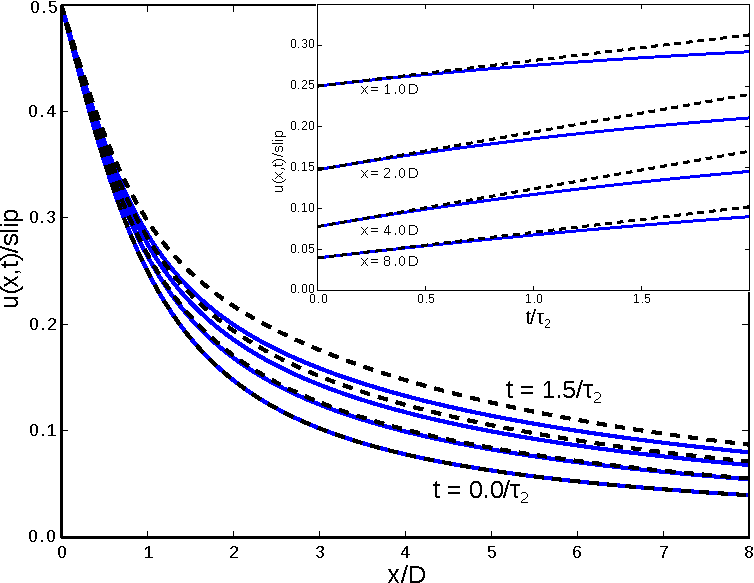
\includegraphics[width=0.8\textwidth]{FinalFigures/Figure1.pdf}
  \caption{Surface displacements predicted by
    eq. (\ref{TwoLayerViscous}) truncated after five terms (blue) and
    the approximation given by eq. (\ref{TwoLayerViscousApprox})
    (dotted black).  Displacements are shown at times 0, 5, 10, and 15
    years following an earthquake}
  \label{figure 1}
\end{figure}

\begin{figure}[h!]\label{figure2}
  \centering
  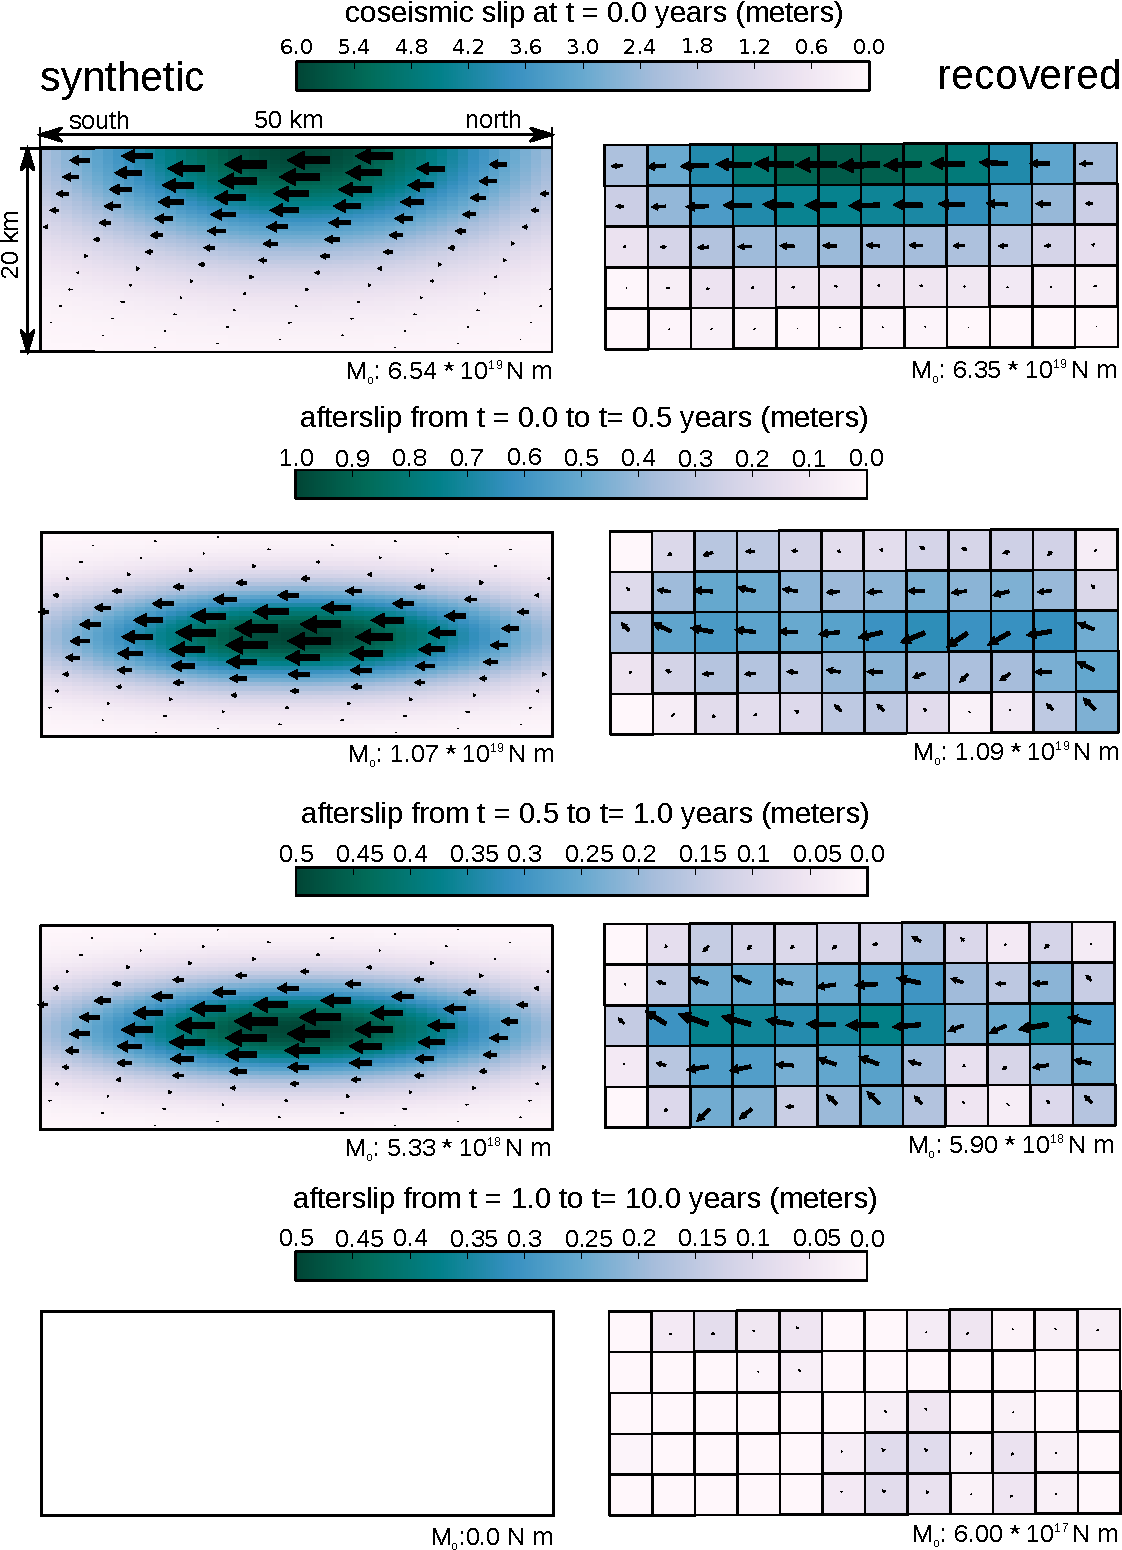
\includegraphics[width=0.9\textwidth]{FinalFigures/Figure2.pdf}
  \caption{Left: slip distribution imposed in the synthetic model.
    The panels from top to bottom represent coseismic slip at time =
    0.0, and afterslip over the period 0.0 to 0.5 years, 0.5 to 1.0
    years, and 1.0 to 10.0 years.  Colors indicate magnitude of slip
    and arrows indicate direction of slip.  Right: Slip recovered from
    inverting the synthetic surface deformation.}
  \label{figure 2}
\end{figure}

\begin{figure}[h!]\label{figure3}
  \centering
  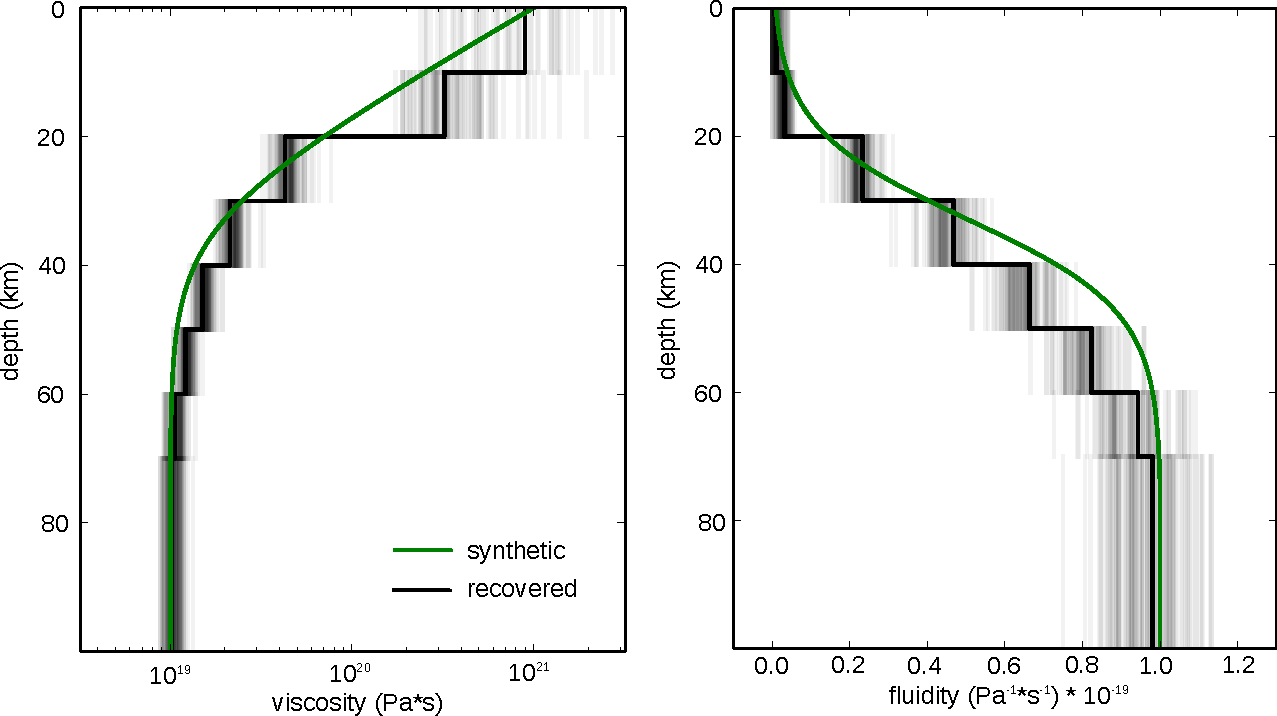
\includegraphics[width=0.9\textwidth]{FinalFigures/Figure3.pdf}
  \caption{Synthetic and recovered lithospheric viscosity strucutures.
    Blue line indicates viscosity structure imposed in the synthetic
    test. Black line indicates viscosity structure inferred from the
    synthetic surface displacement.  Semi-transparent lines are
    recovered models found through bootstrapping and indicate the
    degree of uncertainty on the inferred viscosity structure.  The
    left and right panels show the same information under
    different projections}
  \label{figure 3}
\end{figure}

\begin{figure}[h!]\label{figure4}
  \centering
  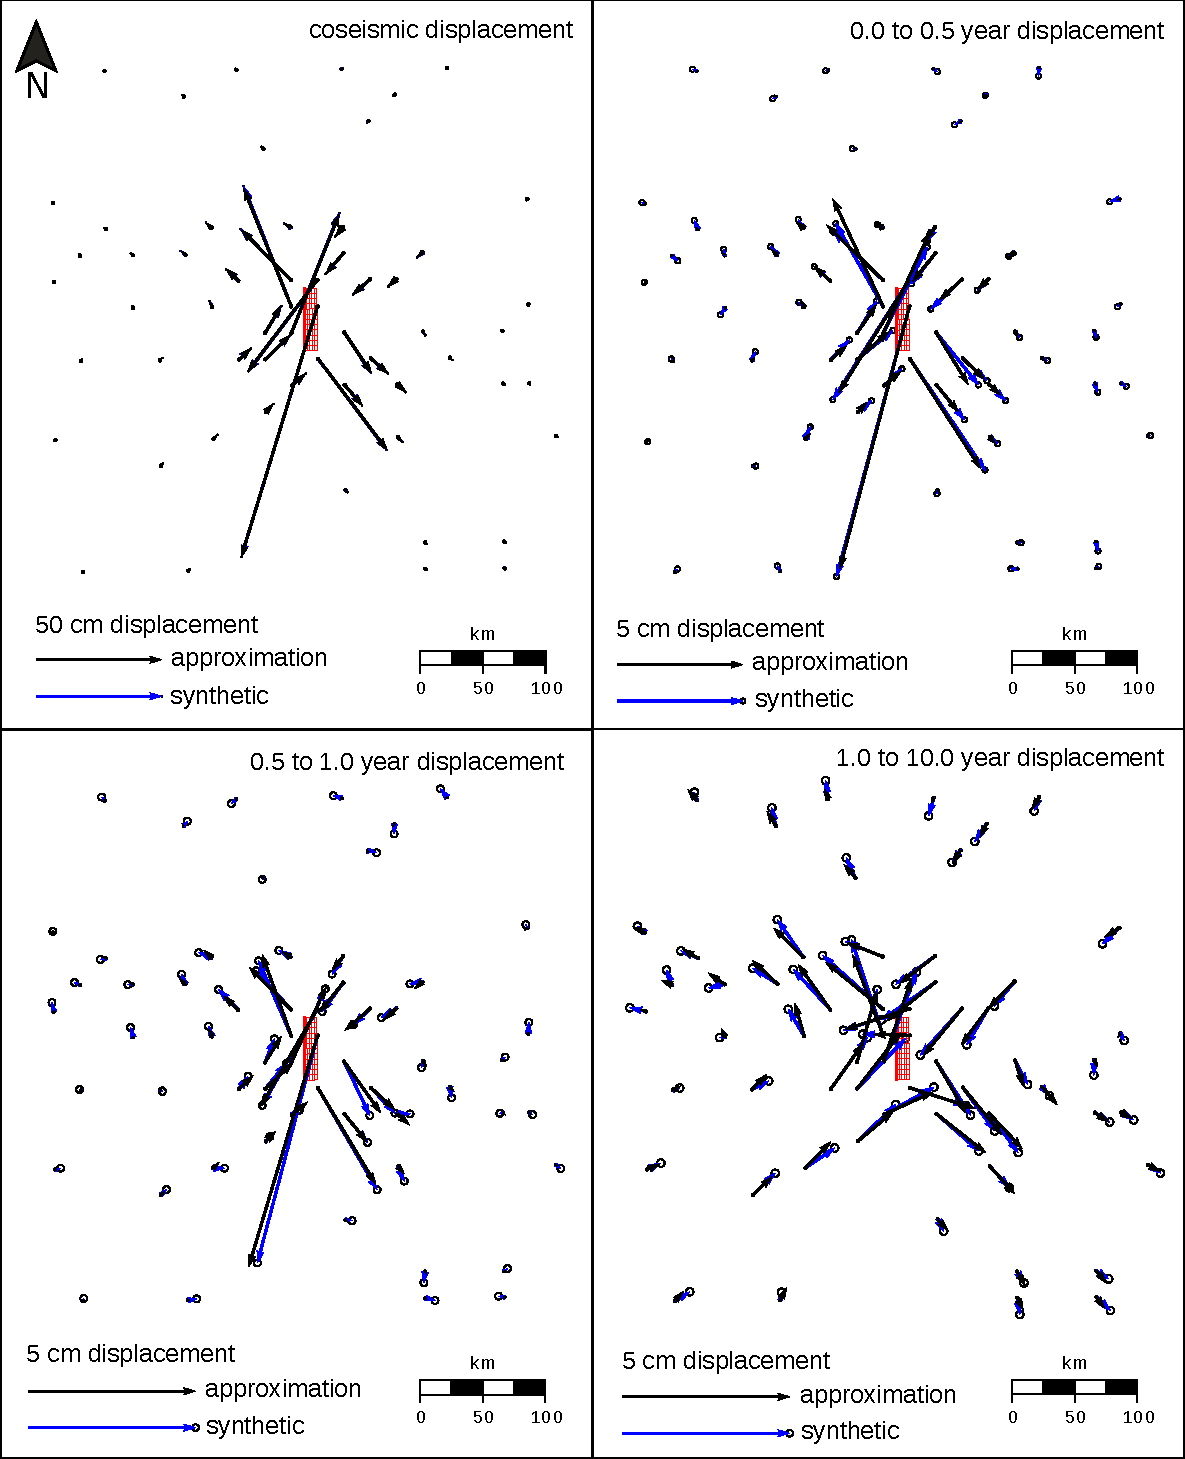
\includegraphics[width=0.9\textwidth]{FinalFigures/Figure4.pdf}
  \caption{Synthetic surface displacements (blue) and best fitting
    surface displacements (black).  Vertical displacements are used in
    the inversion but are not shown here.  The top left panel shows
    coseismic displacements and the remaining panals show the
    displacements over the indicated time intervals. Red dot indicates
    the position whos time series is shown in figure 5. The red wireframe
    is the synthetic fault discretized into fault patches.}
  \label{figure 4}
\end{figure}

\begin{figure}[h!]\label{figure5}
  \centering
  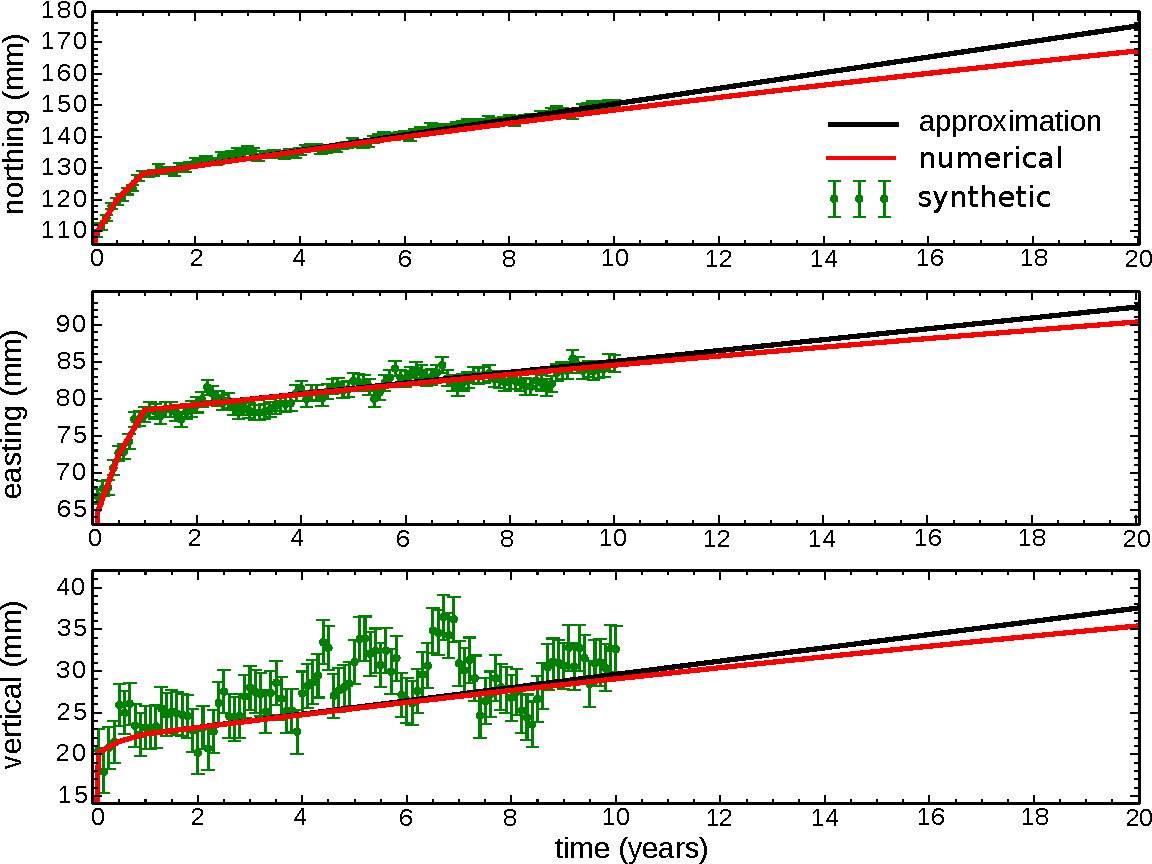
\includegraphics[width=0.9\textwidth]{FinalFigures/Figure5.pdf}
  \caption{Displacement time series for the position shown in figure 4
    (blue) and best fitting surface displacements using the
    approximation from eq. (\ref{Postseismic_Approximation}) (black).
    The red line indicates surface displacements computed using Pylith
    where the inferred slip distribution and viscosity structure are
    used as input. Values for displacement are with respect to the
    locations preseismic position.}  
  \label{figure 5}
\end{figure}

%\begin{figure}[h!]\label{figure6}
%  \centering
%  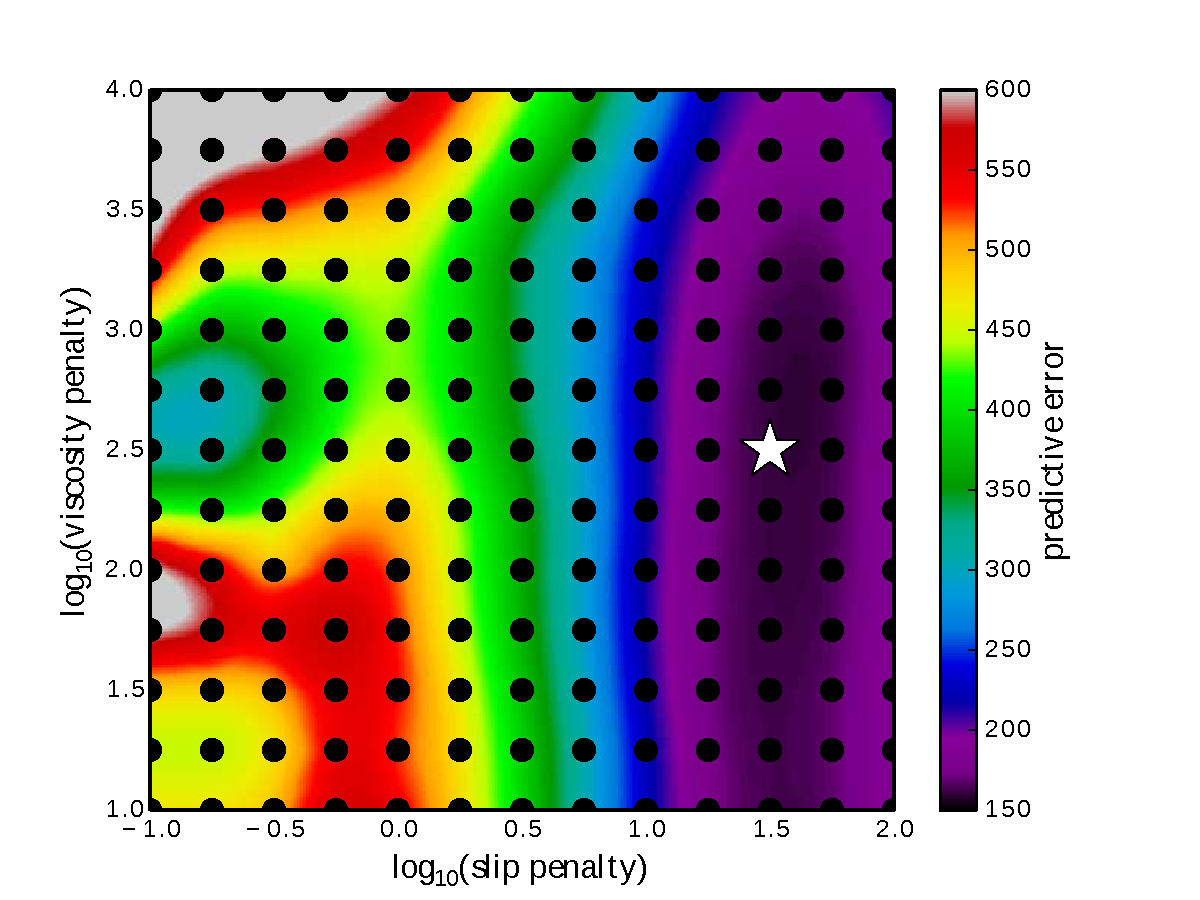
\includegraphics[width=0.9\textwidth]{FinalFigures/Figure6.pdf}
%  \caption{Predictive error for various pairs of slip and viscosity
%    penalty parameters.  Values are interpolated from the predictive
%    errors computed at each of the black dots.  The optimal pair of
%    penalty parameters produce the minimum predictive error and are
%    indicated by the star.}
%  \label{figure 6}
%\end{figure}

\begin{figure}[h!]\label{figure6}
  \centering
  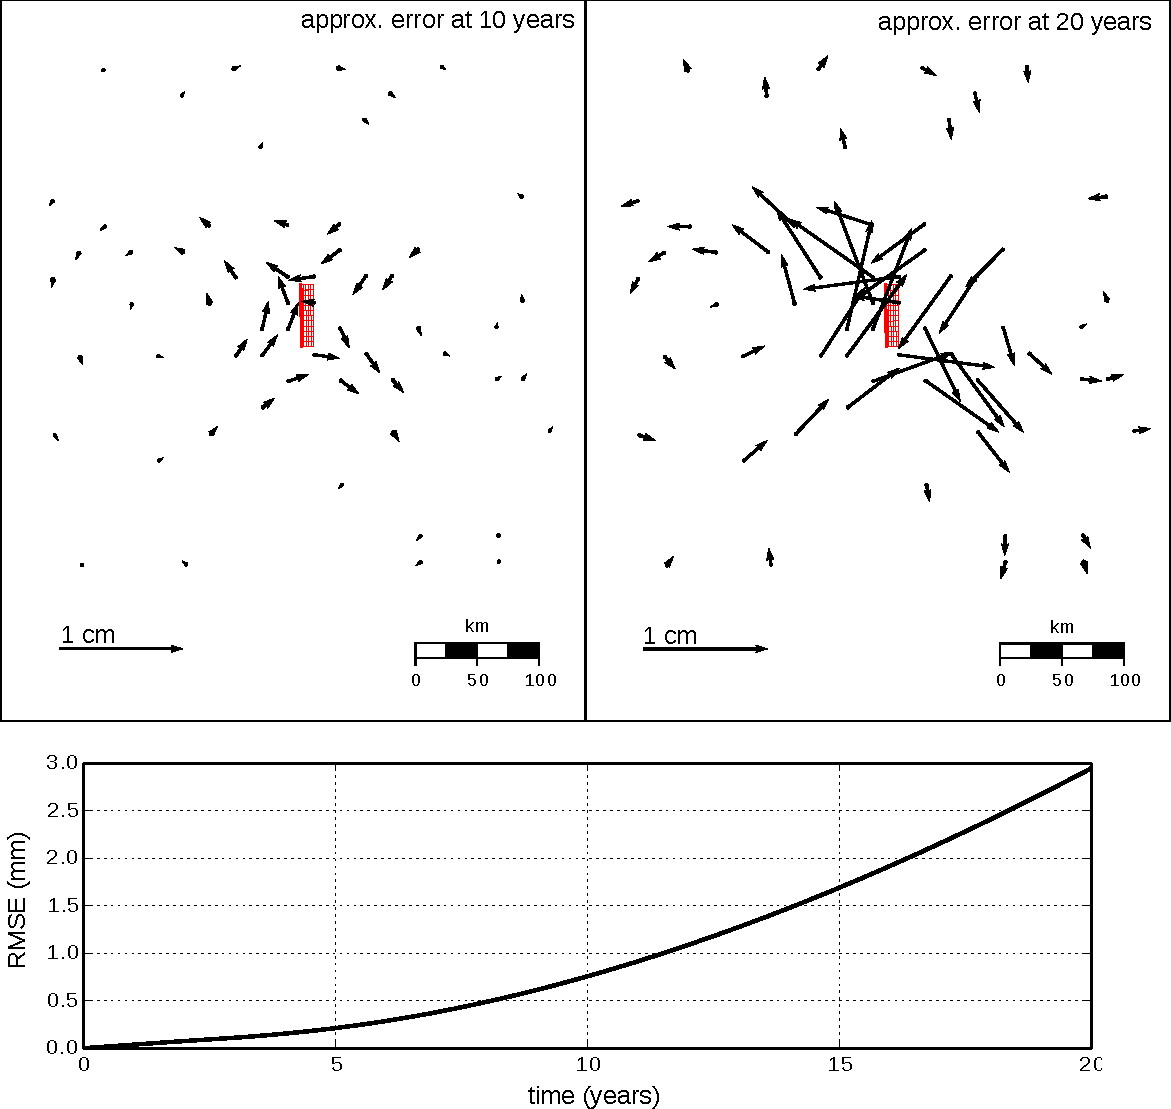
\includegraphics[width=0.9\textwidth]{FinalFigures/Figure7.pdf}
  \caption{Difference between the surface displacement approximation
    and the numerically computed surface displacements.  Top left
    panel shows the difference 10 years after the earthquake and the
    top right panel shows the difference at 20 years.  The bottom
    panel shows the root mean square of the approximation error over
    time.}
  \label{figure 6}
\end{figure}


\end{document}
